\documentclass[12pt]{article}%
\usepackage{amsfonts}
\usepackage{fancyhdr}
\usepackage{comment}
\usepackage[a4paper, top=2.5cm, bottom=2.5cm, left=2.2cm, right=2.2cm]%
{geometry}
\usepackage{times}
\usepackage{amsmath}
\usepackage{changepage}
\usepackage{amssymb}
\usepackage{graphicx}%
\setcounter{MaxMatrixCols}{30}
\newtheorem{theorem}{Theorem}
\newtheorem{acknowledgement}[theorem]{Acknowledgement}
\newtheorem{algorithm}[theorem]{Algorithm}
\newtheorem{axiom}{Axiom}
\newtheorem{case}[theorem]{Case}
\newtheorem{claim}[theorem]{Claim}
\newtheorem{conclusion}[theorem]{Conclusion}
\newtheorem{condition}[theorem]{Condition}
\newtheorem{conjecture}[theorem]{Conjecture}
\newtheorem{corollary}[theorem]{Corollary}
\newtheorem{criterion}[theorem]{Criterion}
\newtheorem{definition}[theorem]{Definition}
\newtheorem{example}[theorem]{Example}
\newtheorem{exercise}[theorem]{Exercise}
\newtheorem{lemma}[theorem]{Lemma}
\newtheorem{notation}[theorem]{Notation}
\newtheorem{problem}[theorem]{Problem}
\newtheorem{proposition}[theorem]{Proposition}
\newtheorem{remark}[theorem]{Remark}
\newtheorem{solution}[theorem]{Solution}
\newtheorem{summary}[theorem]{Summary}
\newenvironment{proof}[1][Proof]{\textbf{#1.} }{\ \rule{0.5em}{0.5em}}

\newcommand{\Q}{\mathbb{Q}}
\newcommand{\R}{\mathbb{R}}
\newcommand{\C}{\mathbb{C}}
\newcommand{\Z}{\mathbb{Z}}

\begin{document}

\title{CS280 Spring 2025 Assignment 2 \\ Part A}
\author{Convolutional Neural Network}
\maketitle

\paragraph{Name: Chen Xuanxin}

\paragraph{Student ID: 2024233125}

\newpage 

\subsubsection*{\textbf{1. CNNs (10 points)}}
Answer the following questions about convolutional neural networks.
\vspace{0.5em}
\\
1. Consider a convolutional layer with 10 filters of size $6 \times 6$, a stride of 2 and a padding of 1. Suppose the input of the layer has shape $64 \times 64 \times 10$ (with spatial size $64 \times 64$ and 10 channels). What is the output shape? What is the number of parameters of the layer (consider the weights and bias)?
\\\\
2. Suppose there are two convolutional layers, each of which has a filter of size $5 \times 5$, a stride of 1, a padding of 0. Is it possible to interpret the result of applying the two convolutional layers successively to an input as the result of applying a single convolutional layer to the input? If so, what is the filter size of the single convolutional layer?   
\\\\
3. Does pooling layers cause loss of information in the inputs? If so, why are pooling layers still used in CNNs (please give at least two reasons)?

\newpage

\subsubsection*{Answer 1}

\textbf{1.} The output shape is given by the formula:

\[
\text{Output size} = \frac{\text{Input size} - \text{Filter size} + 2 \times \text{Padding}}{\text{Stride}} + 1
\]

Thus, we have:

\[
\frac{64 - 6 + 2\times 1}{2} + 1 = \frac{60}{2} + 1 = 31
\]

The output shape is $31 \times 31 \times 10$.

Number of parameters (weights + biases):

Each filter: $6 \times 6 \times 10 = 360$ parameters.  

Total weights for 10 filters: $360 \times 10 = 3600$ parameters.  

Biases for each filter: $10$ parameters.

Therefore, total parameters: $3600 + 10 = 3610$.

\vspace{1em}

\textbf{2.} Yes, it is possible. Two successive convolutional layers, each with filter size $5\times 5$, stride 1 and padding 0, can be represented as a single convolutional layer. The equivalent single convolution filter size will be:

\[
(5 + 5 - 1) \times (5 + 5 - 1) = 9 \times 9
\]

Thus, the equivalent single filter size is $9 \times 9$.

\vspace{1em}

\textbf{3.} Yes, pooling layers do cause loss of information because they aggregate local spatial information. However, pooling layers are still widely used because:

(1) Pooling reduces the spatial dimension of feature maps, significantly decreasing computational cost and memory usage.

(2) Pooling layers provide a form of spatial invariance, making the CNN less sensitive to small translations or variations in input.



\newpage

\subsubsection*{\boldmath{2. Backpropagation of CNNs (10 points)}}
Let $f_w(z)=z*w$ be the forward model for a 2D convolutional layer with a single input channel and a single 
output channel, where $w$ represents a 
$3\times3$ convolution kernel with no padding and a stride of 1, and 
$z$ represents a single-channel $128\times128$ image. \\
The following two functions must be implemented in order to implement 
both the forward pass and backward pass for this single layer:
$$x = F(z, w),$$
$$(g_z, g_w) = G(\epsilon).$$
The figures below illustrate the functions graphically:
\begin{figure}[htbp]
    \centering
    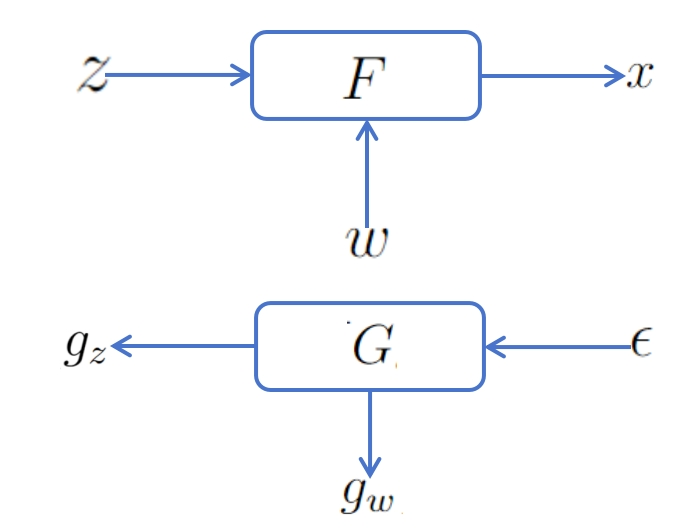
\includegraphics[width=5cm]{examp.png}
\end{figure}

\noindent Answer the following questions:
\vspace{0.5em}
\\
1. Explain what the two functions $F(z, w)$ and $G(\epsilon)$ do. For each function, explain why it is needed. 
\\\\   
2. What are the shapes of each of the following: $x$, $\epsilon$, $g_z$, $g_w$? 
\\\\
3. What is the computational cost (the number of multiplications and additions) of the convolutional layer in forward pass? What is the computational cost (the number of multiplications and additions) of $g_w$ in backward pass?

\newpage

\subsubsection*{Answer 2}

\textbf{1.} My answer is as follows:

Function $F(z, w)$ is the forward convolution function that convolves input image $z$ with kernel $w$ to produce the output feature map $x$. It is necessary because it computes the output activations for forward propagation.

Function $G(\epsilon)$ is the backward convolution (gradient) function. It computes gradients of the loss with respect to inputs $z$ (denoted as $g_z$) and weights $w$ (denoted as $g_w$), given the upstream gradient $\epsilon$. It is needed to perform the backward propagation (training) to update parameters using gradients.

\vspace{1em}

\textbf{2.} Shapes are as follows:

 (1) $x$: $(126, 126)$, since $128 - 3 + 1 = 126$.
 
 (2) $\epsilon$: Same as $x$, thus $(126, 126)$.
 
 (3) $g_z$: Same shape as original input $z$, thus $(128, 128)$.
 
 (4) $g_w$: Same shape as convolution kernel $w$, thus $(3, 3)$.
  
\vspace{1em}

\textbf{3.} My answer is as follows:
\begin{itemize}
 \item \textbf{Forward pass computational cost:}

Output dimension: $126\times126$, each position involves a $3\times3$ convolution operation, thus:

Multiplications per output pixel: $3 \times 3 = 9$  
Additions per output pixel: $9 - 1 = 8$

Total multiplications: $126 \times 126 \times 9 = 142,884$  
Total additions: $126 \times 126 \times 8 = 126,112$

 \item \textbf{Backward pass computational cost for $g_w$:}

Gradient $g_w$ has size $3\times3$. Each parameter of $g_w$ is computed by convolution of input $z$ (size $128\times128$) and gradient $\epsilon$ (size $126\times126$):

Total multiplications: same as forward pass, $126\times126\times9=142,884$  
Total additions: $126\times126\times8=126,112$

\end{itemize}

\end{document}